\documentclass[12pt]{article}
\usepackage[a4paper,headheight=4pt,scale={0.7,0.8},hoffset=0.1cm]{geometry}
\usepackage[pdftex]{graphicx}
%\usepackage[demo]{graphicx}
\usepackage{adjustbox}
\usepackage{amssymb}
%\usepackage[bookmarks,bookmarksopen,bookmarksdepth=2]{hyperref}
\usepackage{color,hyperref}
\definecolor{darkblue}{rgb}{0.0,0.0,0.3}
\hypersetup{breaklinks,colorlinks,
            linkcolor=black,urlcolor=black,
            anchorcolor=black,citecolor=black,
            %linkcolor=darkblue,urlcolor=darkblue,
            %anchorcolor=darkblue,citecolor=darkblue,
            %draft
            }
\title{Tutorial prueba integraci\'on}
%\author{the author}
%\setcounter{tocdepth}{2}%  alternative (2 or higher)
\begin{document}
\maketitle
\clearpage
\section{Pasos para probar contectarse con integraci\'on}

\begin{itemize}
\item Ejecutar: % \newline
\begin{verbatim}
mvn clean package
\end{verbatim}

\begin{minipage}[t]{\linewidth}
          \raggedright
          \adjustbox{valign=t}{%
            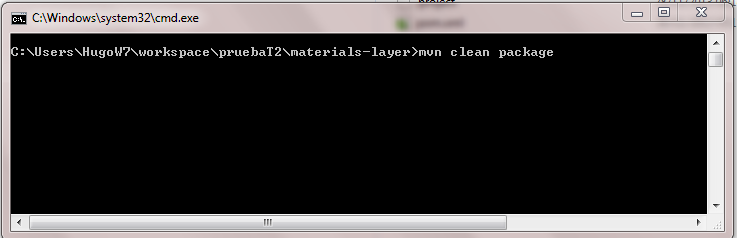
\includegraphics[width=.95\linewidth]{mvnpackage}%
          }

          \medskip
          
    \end{minipage}
\item Verificar: % \newline
\begin{verbatim}
BUILD SUCCESS
\end{verbatim}
\begin{minipage}[t]{\linewidth}
          \raggedright
          \adjustbox{valign=t}{%
            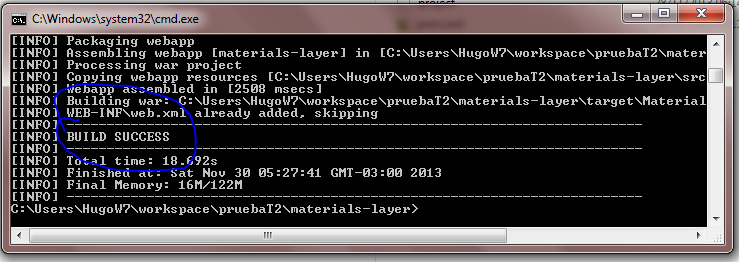
\includegraphics[width=.95\linewidth]{mvnsuccess}%
          }

          \medskip
          \textbf{Si no llegan a esto me avisan lo antes posible}
    \end{minipage}
%\begin{itemize}
\item Ejecutar: % \newline
\begin{verbatim}
 mvn eclipse:eclipse -Dwtpversion=2.0
\end{verbatim}
\item Importar en eclipse este proyecto.
\item este paso es para asegurarnos que anda todo bien. Con el eclipse abierto vuelven a la consola y ejecutan:
\begin{verbatim}
 mvn eclipse:clean
\end{verbatim}
Y en \emph{eclipse} clic derecho sobre el proyecto \emph{Configure $\rightarrow$ Convert to Maven Project}. \newline
Luego, clic derecho sobre el proyecto \emph{Maven $\rightarrow$ Update project.. (Alt + F5) }
\item (dami .. esto creo que yami ya lo tiene y con andy lo hicimos hace un rato) configuren axis2 en eclipse \ \newline
\begin{itemize}
\item bajar  \ \newline
 \textit{\href{http://apache.dattatec.com//axis/axis2/java/core/1.6.2/axis2-1.6.2-bin.zip} {http://apache.dattatec.com//axis/axis2/java/core/1.6.2/axis2-1.6.2-bin.zip}}
\item  descomprimir 
\item seguir estas instrucciones  \ \newline
\textit{\href{http://efunctions.wordpress.com/2011/12/19/configurando-apache-axis2-en-eclipse-indigo/} {http://efunctions.wordpress.com/2011/12/19/configurando-apache-axis2-en-eclipse-indigo/}}
\item \begin{minipage}[t]{\linewidth}
          \raggedright
          \adjustbox{valign=t}{%
            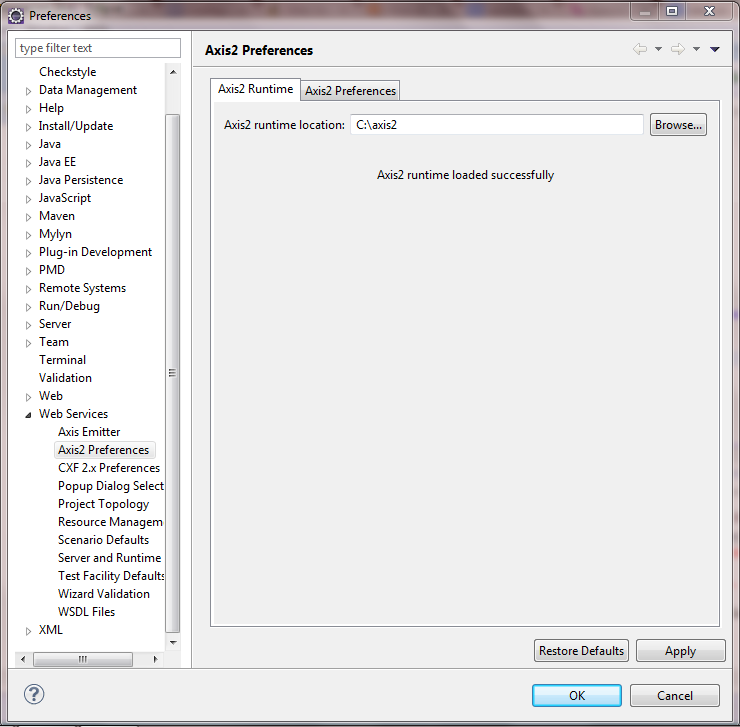
\includegraphics[width=.95\linewidth]{axisconfig}%
          }

          \medskip
          As\'i se ve el m\'io
    \end{minipage}
\item Crear un proyecto "dummy" para que eclipse se entere de que tiene axis2: \ \newline
\begin{itemize}
\item File $\rightarrow$ New.. $\rightarrow$ Dynamic Web Proyect
\item Project name: \textbf{"LoQueSea"} 
\item Dynamic web module version: \textbf{2.5} 
\item Configuration $\rightarrow$ Modify.. $\rightarrow$ tildar \emph{Axis2 Web Services} 
\item Ok $\rightarrow$ Finish
\end{itemize}
\item Detener (si existe y est\'a corriendo por fuera del eclipse) el Tomcat, en linux se usa esto:
\begin{verbatim}
sudo /etc/init.d/tomcat7 stop
\end{verbatim}
\item Buscar dentro de \emph{eclipse} el proyecto \textsc{Servers} y abrirlo.
%\begin{figure}[H]
%\centering
%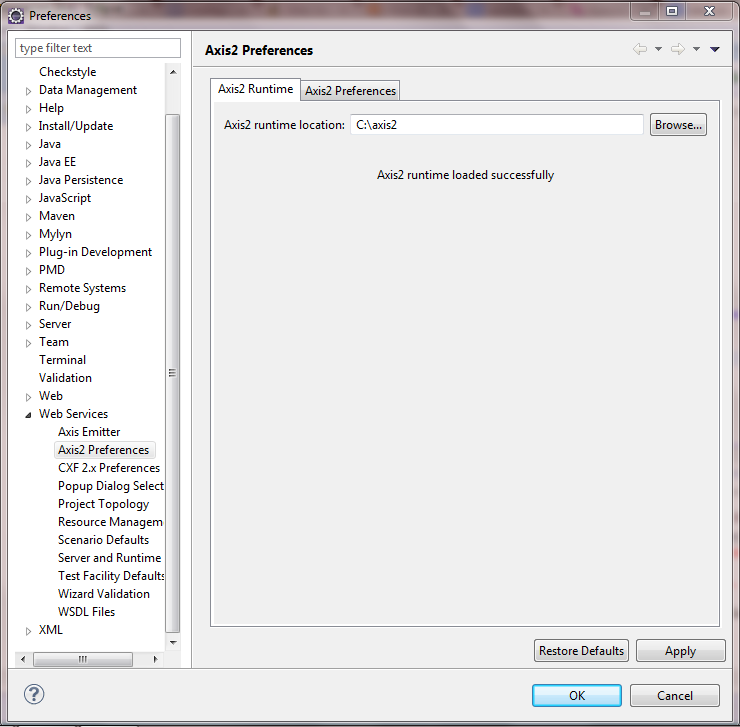
\includegraphics[scale=0.9]{axisconfig}
%%\caption{Balance del per\'iodo}
%%\label{fig:balanc}
%\end{figure} 
\end{itemize}
\item copien la carpeta Integracion2 que est\'a en el repo dentro de su workpace de eclipse
\item importen ese proyecto a eclipse
\item en ese proyecto clic derecho sobre /com/ws/services/IntegracionWS.java
\item New $\rightarrow$  Other..$\rightarrow$ WebServices $\rightarrow$ Web Service
\item  \begin{minipage}[t]{\linewidth}
          \raggedright
          \adjustbox{valign=t}{%
            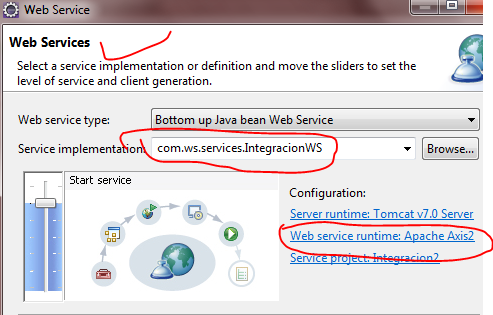
\includegraphics[width=.9\linewidth]{ws}%
          }

          \medskip
          \textbf{As\'i deber\'ia verse, tiene q decir \emph{Apache Axis2}!} \ \newline
          si no dice.. clic y seleccionar Axis2
          
    \end{minipage}
   \item
          En caso de que aparezca algo asi:
            \raggedright
          \adjustbox{valign=t}{%
            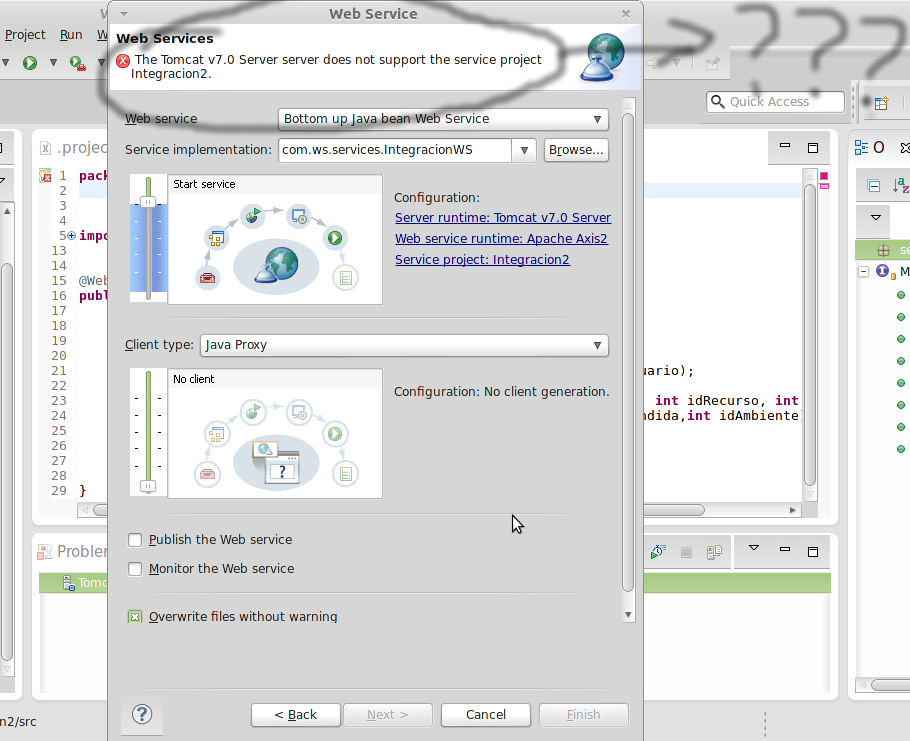
\includegraphics[width=.9\linewidth]{ws2}%
          }

          \medskip
          
          Se deber\'an seguir los siguientes pasos:
          Click derecho sobre el projecto de Integracion2 $\rightarrow$ properties $\rightarrow$  project facets$\rightarrow$ dinamic web module y se reemplaza por 2.5
\item dejar el resto como est\'a y darle siguiente.. siguiente..
\item probarlo... \ \newline
\textit{\href{http://localhost:8080/Integracion2/services/IntegracionWS?wsdl} {http://localhost:8080/Integracion2/services/IntegracionWS?wsdl}}
\item Ahora hay que probar el cliente
\item \begin{minipage}[t]{\linewidth}
          \raggedright
          \adjustbox{valign=t}{%
            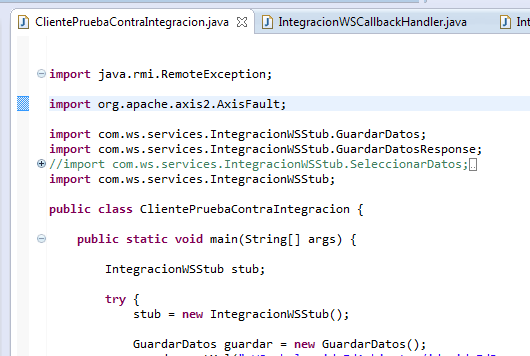
\includegraphics[width=.95\linewidth]{client}%
          }

          \medskip
          \textbf{ejecutar como java application el archivo: \emph{ClientePruebaContraIntegracion.java}} 
    \end{minipage}
    \item \ \newline
    \begin{minipage}[t]{\linewidth}
          \raggedright
          \adjustbox{valign=t}{%
            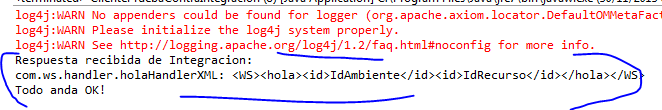
\includegraphics[width=.95\linewidth]{ok}%
          }

          \medskip
          \textbf{les tiene que aparecer esto \emph{(Caso contrario.. me avisan!)}} 
    \end{minipage}
\end{itemize}

\clearpage
\section{Generaci\'on de un cliente de nuestro Web Service}
Se va a hacer un cliente simple en un \emph{main} y se muestran algunas invocaciones de ejemplo.
\begin{itemize}
\item En \emph{eclipse} se crea un proyecto com\'un de Java y llamenlo "ClienteNuestro": \newline
\emph{File $\rightarrow$ New $\rightarrow$  Other..$\rightarrow$ Java Project} \newline
    \begin{minipage}[t]{\linewidth}
          \raggedright
          \adjustbox{valign=t}{%
            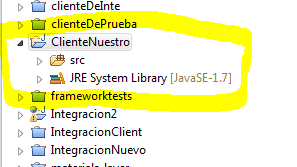
\includegraphics[width=.6\linewidth]{eclipseclient}%
          }

          \medskip
    \end{minipage}
\item Ir a nuestro proyecto y ejecutar como \emph{Java application} la clase \textbf{WSPublisher} y tomar nota de la url en la cual se est\'a publicando el servicio. En la consola se va a ver esto: 
\begin{verbatim}
Ingrese "hola" para salir : 
\end{verbatim}
    \begin{minipage}[t]{\linewidth}
          \raggedright
          \adjustbox{valign=t}{%
            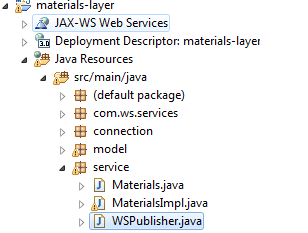
\includegraphics[width=.6\linewidth]{wspubl}%
          }

          \medskip
          \scriptsize En caso de que d\'e alg\'un error: puede ser que el puerto est\'e ocupado y haya que detener eso, aunque ac\'a se puede poner manualmente cualquier puerto cambiando el par\'ametro del m\'etodo \textsc{Endpoint.publish}.
    \end{minipage}
\item Dentro del workspace ir a la carpeta del proyecto y abrir un terminal ah\'i
    \begin{minipage}[t]{\linewidth}
          \raggedright
          \adjustbox{valign=t}{%
            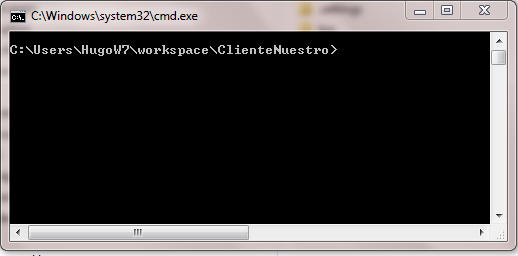
\includegraphics[width=.6\linewidth]{commandline}%
          }

          \medskip
    \end{minipage}
\item Ejecutar el siguiente comando para generar el c\'odigo cliente (la url contiene parte de lo que dice el par\'ametro del m\'etodo \textsc{Endpoint.publish} ):
\begin{verbatim}
wsimport -s src -keep -verbose http://localhost:8081/WS2/Greeting2?wsdl
\end{verbatim}
\item En la pantalla se debe ver algo as\'i
\begin{verbatim}
parsing WSDL...
Generating code...

service\AgregarEncuesta.java
service\AgregarEncuestaRespondida.java
service\AgregarEncuestaRespondidaResponse.java
service\AgregarEncuestaResponse.java
service\AgregarLink.java
service\AgregarLinkResponse.java
.... (todas las clases deben aparecer)

Compiling code...

javac -d ...
\end{verbatim}
{
 \scriptsize En caso de que d\'e alg\'un error: puede ser que est\'a mal la url o el servicio no est\'a levantado }
\item En \emph{eclipse} clic derecho sobre el proyecto "ClienteNuestro"  $\rightarrow$ Refresh
\item Crear una clase Client con este c\'odigo (dejo la clase creada en la carpeta turorial):
\scriptsize
\begin{verbatim}

import java.io.BufferedReader;
import java.io.IOException;
import java.io.InputStreamReader;
import java.util.List;

import service.Encuesta;
import service.Materials;
import service.MaterialsImplService;
import service.Pregunta;

public class Client {

	public static void main(String[] args) {
		MaterialsImplService service = new MaterialsImplService();
		Materials port = service.getMaterialsImplPort();
		System.out.println("------->>  Probando el servicio");
		System.out.println(port.sayHello("Programador"));
		System.out.println("------->>  ESTA TODO OK!");

		System.out.println("Ingrese algo para continuar y probar las encuestas : ");

		try {
			BufferedReader bufferRead = new BufferedReader(new InputStreamReader(System.in));
			bufferRead.readLine();

		} catch (IOException e) {
			e.printStackTrace();
		}

		try {
		Encuesta enc = port.getEncuesta(0, 0);

		System.out.println("TITULO ENCUESTA: " + enc.getDescripcion());

		List<Pregunta> preguntas = enc.getPreguntas();
		for (Pregunta p : preguntas) {
			System.out.println("\t" + p.getEnunciado());
		}
		} catch (Exception e) {
			System.out.println("Encuesta inexistente!");
		}

	}

}
\end{verbatim}
\end{itemize}

%\label{sect:A}
%\subsection{a}
%\subsection{b}
%% ...
%\section{B}
%\label{sect:B}
%\subsection{a}
%\subsection{b}
%% ...
%\section{C}
%\label{sect:C}
%\subsection{a}
%\subsection{b}
% ...
\end{document}